\documentclass{article}
\usepackage{xeCJK}  %必须加xeCJK包
\setCJKmainfont{AR PL UMing CN}  %换成本地字体

% if you need to pass options to natbib, use, e.g.:
% \PassOptionsToPackage{numbers, compress}{natbib}
% before loading nips_2016
%
% to avoid loading the natbib package, add option nonatbib:
% \usepackage[nonatbib]{nips_2016}

\usepackage[final,nonatbib]{nips_2016}

% to compile a camera-ready version, add the [final] option, e.g.:
% \usepackage[final]{nips_2016}

\usepackage[utf8]{inputenc} % allow utf-8 input
\usepackage[T1]{fontenc}    % use 8-bit T1 fonts
\usepackage{hyperref}       % hyperlinks
\usepackage{url}            % simple URL typesetting
\usepackage{booktabs}       % professional-quality tables
\usepackage{amsfonts}       % blackboard math symbols
\usepackage{nicefrac}       % compact symbols for 1/2, etc.
\usepackage{microtype}      % microtypography
\usepackage{amsmath}
\usepackage{graphicx}
\usepackage{subcaption}

% for syntax highlighting of code
\usepackage{xcolor}
\usepackage{listings}

\lstset{
language=Python,
basicstyle=\ttfamily,
otherkeywords={self},             
keywordstyle=\ttfamily\color{blue!90!black},
keywords=[2]{True,False},
keywords=[3]{ttk},
%keywordstyle={[2]\ttfamily\color{yellow!80!orange}},
keywordstyle={[3]\ttfamily\color{red!80!orange}},
emph={MyClass,__init__},          
emphstyle=\ttfamily\color{red!80!black},    
stringstyle=\color{green!80!black},
showstringspaces=false            
}

\title{An overview of gradient descent optimization algorithms\thanks{This paper originally appeared as a blog post at \url{http://sebastianruder.com/optimizing-gradient-descent/index.html} on 19 January 2016.}}

\title{梯度下降类优化算法概述\thanks{本文原载于2016年1月19号的博客 \url{http://sebastianruder.com/optimizing-gradient-descent/index.html}}}

% The \author macro works with any number of authors. There are two
% commands used to separate the names and addresses of multiple
% authors: \And and \AND.
%
% Using \And between authors leaves it to LaTeX to determine where to
% break the lines. Using \AND forces a line break at that point. So,
% if LaTeX puts 3 of 4 authors names on the first line, and the last
% on the second line, try using \AND instead of \And before the third
% author name.

\author{
  Sebastian Ruder\\
  Insight Centre for Data Analytics, NUI Galway\\
  Aylien Ltd., Dublin\\
  \texttt{ruder.sebastian@gmail.com}、、
  翻译:管枫(初),彭博(复),zhangdotcn(审)
}

\begin{document}

\maketitle

\begin{abstract}
Gradient descent optimization algorithms, while increasingly popular, are often used as black-box optimizers, as practical explanations of their strengths and weaknesses are hard to come by. This article aims to provide the reader with intuitions with regard to the behaviour of different algorithms that will allow her to put them to use. In the course of this overview, we look at different variants of gradient descent, summarize challenges, introduce the most common optimization algorithms, review architectures in a parallel and distributed setting, and investigate additional strategies for optimizing gradient descent.

梯度下降类算法在优化问题中非常流行,但是因为难以简单的对众多梯度下降类算法给出一个实用的优劣分析,所以在实际应用中这类算法常常被当作黑箱算法来使用。本文的目的是为读者提供不同算法效果的直观展示,并希望读者能够在实际问题中更合理的选择和使用梯度下降类算法。在这个概述中,我们考察梯度下降算法的不同类型,总结其面临的挑战,介绍几种常用的具体算法,简单介绍并行与分布式架构,并探索其他一些梯度下降类优化策略。
\end{abstract}

\section{Introduction}

Gradient descent is one of the most popular algorithms to perform optimization and by far the most common way to optimize neural networks. At the same time, every state-of-the-art Deep Learning library contains implementations of various algorithms to optimize gradient descent (e.g. lasagne's\footnote{\url{http://lasagne.readthedocs.org/en/latest/modules/updates.html}}, caffe's\footnote{\url{http://caffe.berkeleyvision.org/tutorial/solver.html}}, and keras'\footnote{\url{http://keras.io/optimizers/}} documentation). These algorithms, however, are often used as black-box optimizers, as practical explanations of their strengths and weaknesses are hard to come by.

梯度下降作为最流行的优化算法之一,目前也是神经网络问题中最常用的优化方法。同时每一个最先进的深度学习库里都包含各种算法来优化梯度下降法(比如:lasagne\footnote{\url{http://lasagne.readthedocs.org/en/latest/modules/updates.html}}, caffe\footnote{\url{http://caffe.berkeleyvision.org/tutorial/solver.html}}, and keras\footnote{\url{http://keras.io/optimizers/}} documentation).然而难以合理的解释其优缺点,这些算法通常被当作黑箱算法来使用。

This article aims at providing the reader with intuitions with regard to the behaviour of different algorithms for optimizing gradient descent that will help her put them to use. In Section \ref{sec:gradient_descent_variants}, we are first going to look at the different variants of gradient descent. We will then briefly summarize challenges during training in Section \ref{sec:challenges}. Subsequently, in Section \ref{sec:algos}, we will introduce the most common optimization algorithms by showing their motivation to resolve these challenges and how this leads to the derivation of their update rules. Afterwards, in Section \ref{sec:parallelizing}, we will take a short look at algorithms and architectures to optimize gradient descent in a parallel and distributed setting. Finally, we will consider additional strategies that are helpful for optimizing gradient descent in Section \ref{sec:strategies}.

本文的目的是提供给读者一些用来优化梯度下降的不同算法的效果的直观展示,并希望能够帮助读者在实际问题中更合理的选择和使用梯度下降类算法。第\ref{sec:gradient_descent_variants}节,我们首先考察一下梯度下降算法的几种类型。然后在第\ref{sec:challenges}节中简单总结在使用中容易遇到的问题。接下来在第\ref{sec:algos}节中,我们介绍最常用的几种算法的动机以及其数学实现,并在第\ref{sec:parallelizing}节中简单看一下在并行和分布式环境中,这些算法和框架是如何来优化梯度下降算法的。最后在第\ref{sec:strategies}节中,我们介绍其他一些可以用来优化梯度下降类算法的策略。

Gradient descent is a way to minimize an objective function $J(\theta)$ parameterized by a model's parameters $\theta \in \mathbb{R}^d$ by updating the parameters in the opposite direction of the gradient of the objective function $\nabla_\theta J(\theta)$ w.r.t. to the parameters. The learning rate $\eta$ determines the size of the steps we take to reach a (local) minimum. In other words, we follow the direction of the slope of the surface created by the objective function downhill until we reach a valley.\footnote{If you are unfamiliar with gradient descent, you can find a good introduction on optimizing neural networks at \url{http://cs231n.github.io/optimization-1/}.}

梯度下降法的基本思想是向着目标函数$J(\theta)$梯度的反方向更新模型参数$\theta \in \mathbb{R}^d$,并以此达到最小化目标函数的目的. 并通过定义学习率$\eta$来决定每一次参数更新时步伐的大小。如果把目标函数图像看作一个山丘,梯度下降法就是沿着山坡最陡峭的方向逐级下降直至山谷的过程。\footnote{对于梯度下降不熟悉的同学可以参考\url{http://cs231n.github.io/optimization-1/}.}


\section{Gradient descent variants} \label{sec:gradient_descent_variants}

There are three variants of gradient descent, which differ in how much data we use to compute the gradient of the objective function. Depending on the amount of data, we make a trade-off between the accuracy of the parameter update and the time it takes to perform an update.

针对于在计算目标函数梯度时所使用数据量的不同,梯度下降分为三种类型.具体操作时,我们在参数更新的准确率和执行更新所消耗的时间之间进行权衡,来选用最合适的类型。

%\subsection{Batch gradient descent}
\subsection{批梯度下降}

Vanilla gradient descent, aka batch gradient descent, computes the gradient of the cost function w.r.t. to the parameters $\theta$ for the entire training dataset:

普通(vanilla)梯度下降,又称为批梯度下降,在整个数据集上计算损失函数关于参数$\theta$的梯度:

\begin{equation}
\theta = \theta - \eta \cdot \nabla_\theta J( \theta)
\end{equation}

As we need to calculate the gradients for the whole dataset to perform just \emph{one} update, batch gradient descent can be very slow and is intractable for datasets that do not fit in memory. Batch gradient descent also does not allow us to update our model \emph{online}, i.e. with new examples on-the-fly.

由于在批梯度下降中为了执行一次更新,我们需要在整个数据集上计算梯度,因此这将会是很慢的,并且内存也是一个棘手的问题.批梯度下降同样也不适用于在线更新我们的模型,例如使用新的样例on-the-fly.

In code, batch gradient descent looks something like this:

在代码中,批梯度下降形如此:

\begin{lstlisting}[language=python]
for i in range(nb_epochs):
  params_grad = evaluate_gradient(loss_function, data, params)
  params = params - learning_rate * params_grad
\end{lstlisting}

For a pre-defined number of epochs,  we first compute the gradient vector \lstinline{params_grad} of the loss function for the whole dataset w.r.t. our parameter vector \lstinline{params}.  Note that state-of-the-art deep learning libraries provide automatic differentiation that efficiently computes the gradient w.r.t. some parameters. If you derive the gradients yourself, then gradient checking is a good idea.\footnote{Refer to \url{http://cs231n.github.io/neural-networks-3/} for some great tips on how to check gradients properly.}

对于预先确定的迭代次数\lstinline{nb_epochs},在每一次迭代中,我们首先在整个数据集上计算损失函数关于模型参数向量\lstinline{params}的梯度\lstinline{params_grad}. 最先进的深度学习代码库都会提供计算梯度的工具,但是如果使用者使用自己的梯度计算工具的话,最好使用梯度检查\footnote{梯度检查请参考 \url{http://cs231n.github.io/neural-networks-3/}}确保不会出错。

We then update our parameters in the direction of the gradients with the learning rate determining how big of an update we perform. Batch gradient descent is guaranteed to converge to the global minimum for convex error surfaces and to a local minimum for non-convex surfaces.

然后我们向着梯度相反的方向更新参数,并利用学习率(\lstinline{learning rate})来决定更新步伐的大小。批梯度下降对于凸函数确保收敛于全局最小值,而对于非凸函数确保收敛于局部最小值。

%\subsection{Stochastic gradient descent}
\subsection{随机梯度下降法}

Stochastic gradient descent (SGD) in contrast performs a parameter update for \emph{each} training example $x^{(i)}$ and label $y^{(i)}$:

与批梯度下降不同,随机梯度下降法(SGD)每一次参数更新时只使用一个样本$x^{(i)}$以及其对应的标注$y^{(i)}$:

\begin{equation}
\theta = \theta - \eta \cdot \nabla_\theta J( \theta; x^{(i)}; y^{(i)})
\end{equation}

Batch gradient descent performs redundant computations for large datasets, as it recomputes gradients for similar examples before each parameter update. SGD does away with this redundancy by performing one update at a time. It is therefore usually much faster and can also be used to learn online.

在样本数量极大的时候,批梯度下降法在每一次参数更新前,要对大量相似的样本计算其损失函数的梯度,这造成很多冗余的计算。SGD 有效避免了这种冗余,所以他通常比较快,而且适用于样本的在线更新(对于在线添加的样本,可以方便的直接带入迭代之中)

SGD performs frequent updates with a high variance that cause the objective function to fluctuate heavily as in Figure \ref{fig:sgd_fluctuation}.

如图\ref{fig:sgd_fluctuation}所示,SGD 频繁更新参数,并使得目标函数值在剧烈震荡中逐步下降。

\begin{figure}
	\centering
  	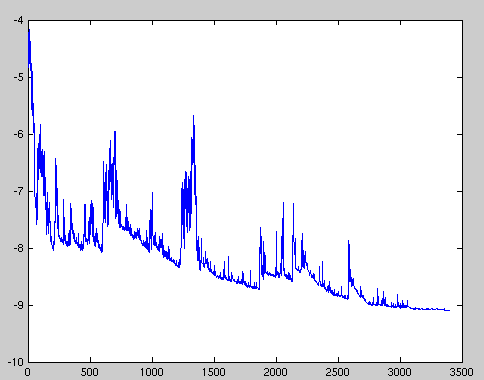
\includegraphics[width=0.4\linewidth]{images/sgd_fluctuation.png}
  	\caption{SGD fluctuation (Source: \href{
https://upload.wikimedia.org/wikipedia/commons/f/f3/Stogra.png}{Wikipedia})}
  	\label{fig:sgd_fluctuation}
\end{figure}

While batch gradient descent converges to the minimum of the basin the parameters are placed in, SGD's fluctuation, on the one hand, enables it to jump to new and potentially better local minima. On the other hand, this ultimately complicates convergence to the exact minimum, as SGD will keep overshooting. However, it has been shown that when we slowly decrease the learning rate, SGD shows the same convergence behaviour as batch gradient descent, almost certainly converging to a local or the global minimum for non-convex and convex optimization respectively.
Its code fragment simply adds a loop over the training examples and evaluates the gradient w.r.t. each example. Note that we shuffle the training data at every epoch as explained in Section \ref{sec:shuffling}.

相对比于批梯度下降法在参数空间中收敛于局部最小值的的表现来说,SGD的高震荡性,一方面使迭代有可能跳出当前的局部最小值并找到更好的局部最小值,另一方面却因为过于活跃而使得收敛变得异常困难。但是,已知的结果显示,只要在迭代中逐渐缩小学习率,那么SGD也会展现出和批梯度下降法类似的收敛效果——分别在凸函数和非凸函数的情形下收敛于整体极小值和局部极小值。在代码上,仅仅是关于训练样本增加了一个子循环来计算关于每一个样本的梯度。请注意我们在每一个外层迭代开始时随机打乱了样本顺序,关于这种技巧我们在第\ref{sec:shuffling}节进行详细介绍。

\begin{lstlisting}[language=python]
for i in range(nb_epochs):
  np.random.shuffle(data)
  for example in data:
    params_grad = evaluate_gradient(loss_function, example, params)
    params = params - learning_rate * params_grad
\end{lstlisting}

%\subsection{Mini-batch gradient descent}
\subsection{小批量梯度下降}

Mini-batch gradient descent finally takes the best of both worlds and performs an update for every mini-batch of $n$ training examples:

最后小批量梯度下降法集中了前述两种方法的优点,每一次参数更新时,都使用一个含有$n$个样本的小批量来计算损失函数的剃度。

\begin{equation}
\theta = \theta - \eta \cdot \nabla_\theta J( \theta; x^{(i:i+n)}; y^{(i:i+n)})
\end{equation}

This way, it a) reduces the variance of the parameter updates, which can lead to more stable convergence; and b) can make use of highly optimized matrix optimizations common to state-of-the-art deep learning libraries that make computing the gradient w.r.t. a mini-batch very efficient. Common mini-batch sizes range between $50$ and $256$, but can vary for different applications. Mini-batch gradient descent is typically the algorithm of choice when training a neural network and the term SGD usually is employed also when mini-batches are used. Note: In modifications of SGD in the rest of this post, we leave out the parameters $x^{(i:i+n)}; y^{(i:i+n)}$ for simplicity.

这种方法,a) 降低了SGD中参数更新的剧烈震荡,所以收敛效果更好, b) 可以很高效的利用目前最先进的深度学习代码库中那些已经得到了高度优化的矩阵运算工具。通常,根据不同的应用场景,小批量的大小取在$50$到$256$之间。目前在神经网络的训练中经常使用小批量梯度下降法,并习惯性的称之为随机梯度下降法(SGD)。注:为了记号方便,在下文SGD改进版本的公式书写中,我们将省略$x^{(i:i+n)}; y^{(i:i+n)}$。

In code, instead of iterating over examples, we now iterate over mini-batches of size $50$:

在下面的代码中,与SGD每次使用一个样本相比而言,小批量梯度下降法每次使用一个大小为$50$的小批量。

\begin{lstlisting}[language=python]
for i in range(nb_epochs):
  np.random.shuffle(data)
  for batch in get_batches(data, batch_size=50):
    params_grad = evaluate_gradient(loss_function, batch, params)
    params = params - learning_rate * params_grad
\end{lstlisting}

%\section{Challenges} \label{sec:challenges}
\section{问题与挑战} \label{sec:challenges}

Vanilla mini-batch gradient descent, however, does not guarantee good convergence, but offers a few challenges that need to be addressed:

然而普通的小批量梯度下降法的收敛性仍然不太好,而且有如下的一些问题需要解决:

\begin{itemize}
\item Choosing a proper learning rate can be difficult. A learning rate that is too small leads to painfully slow convergence, while a learning rate that is too large can hinder convergence and cause the loss function to fluctuate around the minimum or even to diverge.
\item 很难选取一个合适的学习率。过小的学习率使得收敛极其缓慢,而过大的学习率会使损失函数在极小值附近剧烈震荡,甚至导致发散。
\item Learning rate schedules \cite{Robbins1951} try to adjust the learning rate during training by e.g. annealing, i.e. reducing the learning rate according to a pre-defined schedule or when the change in objective between epochs falls below a threshold. These schedules and thresholds, however, have to be defined in advance and are thus unable to adapt to a dataset's characteristics \cite{Darken1992}.
\item 预定学习率衰减\cite{Robbins1951}的方法可以在训练过程中调整学习率,比如按照一开始定义好的计划逐渐削减学习率或者当相邻的两次迭代中目标函数的变化小于某一个阈值时减小学习率。但是这些计划和阈值都必须要在训练前就定义好,所以无法达到为训练样本量身定做的效果。
\item Additionally, the same learning rate applies to all parameter updates. If our data is sparse and our features have very different frequencies, we might not want to update all of them to the same extent, but perform a larger update for rarely occurring features.
\item 另外,所有的参数更新都使用了同样的学习率。如果数据具有稀疏性而且不同的特征出现的频率有很大差异时,我们更希望对那些极少出现的特征使用较大的学习率,而不是对大家一视同仁。
\item Another key challenge of minimizing highly non-convex error functions common for neural networks is avoiding getting trapped in their numerous suboptimal local minima. Dauphin et al. \cite{Dauphin2014} argue that the difficulty arises in fact not from local minima but from saddle points, i.e. points where one dimension slopes up and another slopes down. These saddle points are usually surrounded by a plateau of the same error, which makes it notoriously hard for SGD to escape, as the gradient is close to zero in all dimensions.
\item 另一个重要的问题是在神经网络的训练中,经常会遇到极为非凸的目标函数,此时很难避免参数被困在一些次优的局部极小值附近。Dauphin et al. \cite{Dauphin2014} 提出这类问题主要发生在鞍点附近。这些鞍点经常环绕着一些平原区域,而在这些区域中,损失函数的梯度很接近于零,所以SGD很难从中逃脱。
\end{itemize}

%\section{Gradient descent optimization algorithms} \label{sec:algos}
\section{随机梯度下降优化算法} \label{sec:algos}

In the following, we will outline some algorithms that are widely used by the Deep Learning community to deal with the aforementioned challenges. We will not discuss algorithms that are infeasible to compute in practice for high-dimensional data sets, e.g. second-order methods such as Newton's method\footnote{\url{https://en.wikipedia.org/wiki/Newton\%27s_method_in_optimization}}.

下面我们介绍一些优化梯度下降算法,他们经常在深度学习中被用来处理上节所提到的问题和挑战。在此我们不讨论那些不适用于高维数据的方法,比如类似于牛顿法\footnote{\url{https://en.wikipedia.org/wiki/Newton\%27s_method_in_optimization}}的二阶算法。

%\subsection{Momentum}
\subsection{动量法}

SGD has trouble navigating ravines, i.e. areas where the surface curves much more steeply in one dimension than in another \cite{Sutton1986}, which are common around local optima. In these scenarios, SGD oscillates across the slopes of the ravine while only making hesitant progress along the bottom towards the local optimum as in Figure \ref{fig:sgd_without_momentum}.

SGD 那种在一个方向上很陡峭而在其他方向上比较平坦,形如峡谷的函数上表现差强人意\cite{Sutton1986},而这种形状在局部极值附近却比较常见。在这种情况下,SGD经常如下图所描述的那样,在峡谷的两边震荡而不能顺利的沿着峡谷方向直接前往最优点。

\begin{figure}[!htb]
    \centering
    \begin{subfigure}{.5\textwidth}
        \centering
        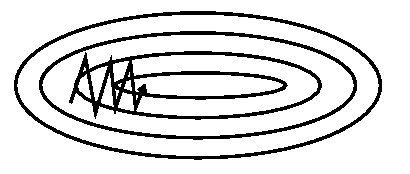
\includegraphics[width=0.8\linewidth]{images/without_momentum.png}
        \caption{SGD without momentum}
        \label{fig:sgd_without_momentum}
    \end{subfigure}%
    \begin{subfigure}{0.5\textwidth}
        \centering
        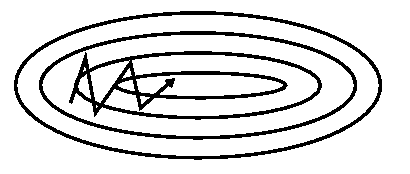
\includegraphics[width=0.8\linewidth]{images/with_momentum.png}
        \caption{SGD with momentum}
        \label{fig:sgd_with_momentum}
    \end{subfigure}
    \caption{Source: \href{https://www.willamette.edu/~gorr/classes/cs449/momrate.html}{Genevieve B. Orr}}
\end{figure}

Momentum \cite{Qian1999} is a method that helps accelerate SGD in the relevant direction and dampens oscillations as can be seen in Figure \ref{fig:sgd_with_momentum}. It does this by adding a fraction $\gamma$ of the update vector of the past time step to the current update vector\footnote{Some implementations exchange the signs in the equations.}

如图\ref{fig:sgd_with_momentum}所示,动量法\cite{Qian1999}可以通过消减这种无谓的震动来加速SGD。动量法的基本原理是在当前的参数更新向量上添加之前一次参数更新向量的一部分\footnote{有些算法实现中会采取不同的符号.}。

\begin{align}
\begin{split}
v_t &= \gamma v_{t-1} + \eta \nabla_\theta J( \theta)\\
\theta &= \theta - v_t
\end{split}
\end{align}

The momentum term $\gamma$ is usually set to $0.9$ or a similar value.

动量项$\gamma$通常被定在$0.9$左右。

Essentially, when using momentum, we push a ball down a hill. The ball accumulates momentum as it rolls downhill, becoming faster and faster on the way (until it reaches its terminal velocity, if there is air resistance, i.e. $\gamma < 1$). The same thing happens to our parameter updates: The momentum term increases for dimensions whose gradients point in the same directions and reduces updates for dimensions whose gradients change directions. As a result, we gain faster convergence and reduced oscillation.

动量法本质上就像是从山顶推一个球下山。球在向下滚动的过程中积累动量速度越来越快(如果存在空气阻力时,也就是$\gamma < 1$的情况,最终会达到平衡速度)。我们的参数更新也是同样的情况: 动量项在那些梯度符号比较一致的方向上不断积累,而在那些梯度经常改变符号的方向上相互抵销,这帮助我们降低震荡从而加快迭代收敛速度。

\subsection{Nesterov accelerated gradient}

However, a ball that rolls down a hill, blindly following the slope, is highly unsatisfactory. We would like to have a smarter ball, a ball that has a notion of where it is going so that it knows to slow down before the hill slopes up again.

但是一个从山顶滚下越滚越快的球并不能满足我们的需求,我们希望这个球更加聪明一些,使得它在到达底部并再次上升之前就开始自动减速。

Nesterov accelerated gradient (NAG) \cite{Nesterov} is a way to give our momentum term this kind of prescience. We know that we will use our momentum term $\gamma \: v_{t-1}$ to move the parameters $\theta$. Computing $\theta - \gamma \: v_{t-1}$ thus gives us an approximation of the next position of the parameters (the gradient is missing for the full update), a rough idea where our parameters are going to be. We can now effectively look ahead by calculating the gradient not w.r.t. to our current parameters $\theta$ but w.r.t. the approximate future position of our parameters:

Nesterov accelerated gradient (NAG) \cite{Nesterov} 就可以赋予我们的动量项这样的先见之明。因为我们知道在第$t$次更新中将会用到动量项$\gamma \: v_{t-1}$, 所以$\theta - \gamma \: v_{t-1}$就给出了参数向量下一个位置的粗略估计。所以我们与其在$\theta$处计算梯度,还不如在这个粗略估计的下一个位置计算梯度。

\begin{align}
\begin{split}
v_t &= \gamma \: v_{t-1} + \eta \nabla_\theta J( \theta - \gamma v_{t-1})\\
\theta &= \theta - v_t
\end{split}
\end{align}

Again, we set the momentum term $\gamma$ to a value of around $0.9$. While Momentum first computes the current gradient (small blue vector in Figure \ref{fig:nesterov update}) and then takes a big jump in the direction of the updated accumulated gradient (big blue vector), NAG first makes a big jump in the direction of the previous accumulated gradient (brown vector), measures the gradient and then makes a correction (green vector). This anticipatory update prevents us from going too fast and results in increased responsiveness, which has significantly increased the performance of RNNs on a number of tasks \cite{Bengio2012a}.\footnote{Refer to \url{http://cs231n.github.io/neural-networks-3/} for another explanation of the intuitions behind NAG, while Ilya Sutskever gives a more detailed overview in his PhD thesis \cite{Sutskever2013a}.}

我们仍然把$\gamma$定为 $0.9$左右。普通的动量法先计算当前的梯度(图\ref{fig:nesterov update}中的短蓝向量),然后沿着累积梯度方向做一个大幅度的参数更新(图中的长蓝向量)。NAG 首先在前一次的累积梯度方向做一个大幅更新(棕色向量),然后再计算梯度,并进行修正(绿色向量)。这种有先见之明的更新方式,可以避免我们更新的幅度过大。这种方法在若干个例子中都显著提升了RNN网络的表现\cite{Bengio2012a}。\footnote{在文章\url{http://cs231n.github.io/neural-networks-3/}中描述了NAG的另一种解释, Ilya Sutskever 在他的博士论文中也给出了详细的介绍 \cite{Sutskever2013a}.}

Now that we are able to adapt our updates to the slope of our error function and speed up SGD in turn, we would also like to adapt our updates to each individual parameter to perform larger or smaller updates depending on their importance.

现在我们可以让我们的参数更新自动适应误差函数的斜率,并确实加速了SGD的收敛。但是另一方面,我们也希望能够让我们的参数更新适应每一个参数,根据他们各自的重要性来决定每一个更新的幅度大小。

\begin{figure}
	\centering
  	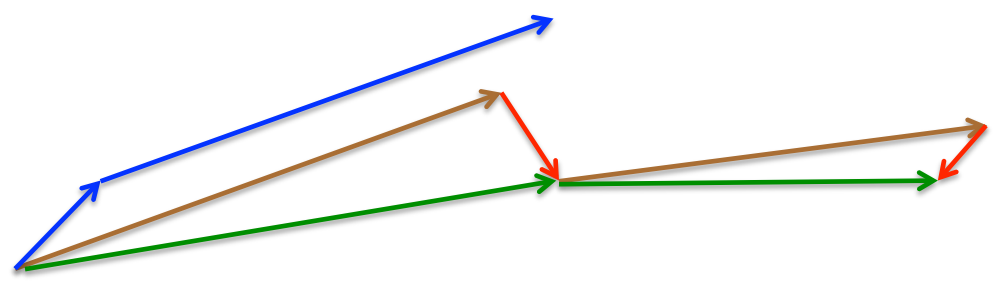
\includegraphics[width=0.4\linewidth]{images/nesterov_update_vector.png}
  	\caption{Nesterov update (Source: \href{
http://www.cs.toronto.edu/~tijmen/csc321/slides/lecture_slides_lec6.pdf}{G. Hinton's lecture 6c})}
  	\label{fig:nesterov update}
\end{figure}

\subsection{Adagrad}

Adagrad \cite{Duchi2011} is an algorithm for gradient-based optimization that does just this: It adapts the learning rate to the parameters, performing larger updates for infrequent and smaller updates for frequent parameters. For this reason, it is well-suited for dealing with sparse data. Dean et al. \cite{Dean2012} have found that Adagrad greatly improved the robustness of SGD and used it for training large-scale neural nets at Google, which -- among other things -- learned to recognize cats in Youtube videos\footnote{\url{http://www.wired.com/2012/06/google-x-neural-network/}}. Moreover, Pennington et al. \cite{Pennington2014} used Adagrad to train GloVe word embeddings, as infrequent words require much larger updates than frequent ones.

Adagrad \cite{Duchi2011} 恰是如此:他是一种可以根据参数的重要性来调整学习率的算法,对于常常更新的参数使用较小的学习率,而对于很少得到更新的参数使用较大的学习率。所以这种方法很适合于稀疏性很强的数据集。 Dean et al. \cite{Dean2012} 发现Adarad 可以大大提升SGD的鲁棒性,于是将其应用于Google的大规模神经网络训练中,并和其他的算法一起实现了在YouTube视频中对猫的自动识别\footnote{\url{http://www.wired.com/2012/06/google-x-neural-network/}}。另外Pennington et al. \cite{Pennington2014}使用Adagrad 对GloVe 词语嵌入进行训练,因为在这种情况下不常出现的词语需要比经常出现的词语更大的学习率。

Previously, we performed an update for all parameters $\theta$ at once as every parameter $\theta_i$ used the same learning rate $\eta$. As Adagrad uses a different learning rate for every parameter $\theta_i$ at every time step $t$, we first show Adagrad's per-parameter update, which we then vectorize. For brevity, we set $g_{t, i}$ to be the gradient of the objective function w.r.t. to the parameter $\theta_i$ at time step $t$:

前面的方法中,我们每一次都用相同的学习率$\eta$对所有参数$\theta_i$进行同步更新。而Adagrad 在每一次更新中都对不同的参数采取不同的学习率,我们首先单独考察每一个参数的更新,然后再将其向量化。简单来说,我们用$g_{t, i}$表示目标函数在第$t$步迭代时,关于参数$\theta_i$的梯度。

\begin{equation}
g_{t, i} = \nabla_\theta J( \theta_i )
\end{equation}

The SGD update for every parameter $\theta_i$ at each time step $t$ then becomes:

SGD对于参数$\theta_i$在第$t$步的更新如下所示:

\begin{equation}
\theta_{t+1, i} = \theta_{t, i} - \eta \cdot g_{t, i}
\end{equation}

In its update rule, Adagrad modifies the general learning rate $\eta$ at each time step $t$ for every parameter $\theta_i$ based on the past gradients that have been computed for $\theta_i$:

而Adagrad在每一次更新时,都针对每一个参数$\theta_i$利用这个参数以往的方向导数值来动态调整其专属的学习率$\eta$:

\begin{equation}
\theta_{t+1, i} = \theta_{t, i} - \frac{\eta}{\sqrt{G_{t, ii} + \epsilon}} \cdot g_{t, i}
\end{equation}

$G_{t} \in \mathbb{R}^{d \times d} $ here is a diagonal matrix where each diagonal element $i, i$ is the sum of the squares of the gradients w.r.t. $\theta_i$ up to time step $t$\footnote{Duchi et al. \cite{Duchi2011} give this matrix as an alternative to the \emph{full} matrix containing the outer products of all previous gradients, as the computation of the matrix square root is infeasible even for a moderate number of parameters $d$.}, while $\epsilon$ is a smoothing term that avoids division by zero (usually on the order of $1e-8$). Interestingly, without the square root operation, the algorithm performs much worse.

此处$G_{t} \in \mathbb{R}^{d \times d} $是一个对角矩阵,其每一个对角元素$i, i$是在以往更新中到第$t$步为止,目标函数在$\theta_i$方向上的导数的平方和。\footnote{Duchi et al. \cite{Duchi2011} 使用这个对角矩阵取代了完整的以往参数更新的协方差矩阵,因为对整个高维矩阵进行开方运算不划算。}, 公式中的$\epsilon$是一个平滑项,用来避免分母为零的情况发生,$\epsilon$通常取值在$1e-8$量级上。有意思的是,如果去掉取平方根那一步,这个算法的表现就会立刻变差很多。

As $G_{t}$ contains the sum of the squares of the past gradients w.r.t. to all parameters $\theta$ along its diagonal, we can now vectorize our implementation by performing an element-wise matrix-vector multiplication $\odot$ between $G_{t}$ and $g_{t}$:

因为 $G_{t}$ 包含了所有参数的以往方向导数的平方和,我们可以很容易的通过$G_{t}$和$g_{t}$之间元素级的矩阵——向量乘法$\odot$来写出这个算法的向量形式:

\begin{equation}
\theta_{t+1} = \theta_{t} - \frac{\eta}{\sqrt{G_{t} + \epsilon}} \odot g_{t}.
\end{equation}

One of Adagrad's main benefits is that it eliminates the need to manually tune the learning rate. Most implementations use a default value of $0.01$ and leave it at that.

Adagrad方法的一个主要的好处是它不需要手动调整学习率。大部分算法实现直接使用默认值$0.01$就好了。

Adagrad's main weakness is its accumulation of the squared gradients in the denominator: Since every added term is positive, the accumulated sum keeps growing during training. This in turn causes the learning rate to shrink and eventually become infinitesimally small, at which point the algorithm is no longer able to acquire additional knowledge. The following algorithms aim to resolve this flaw.

Adagrad 方法的主要弱点是它会在分母上不断累积梯度平方和:因为每次加入的都是正数,所以分母随着训练步骤增加不断变大。这就使得学习率不断衰减,直到接近无限小(指趋近于0),以至于参数更新无法继续前进。下面这个算法就是针对于此的一个改进。

\subsection{Adadelta}

Adadelta \cite{Zeiler2012} is an extension of Adagrad that seeks to reduce its aggressive, monotonically decreasing learning rate. Instead of accumulating all past squared gradients, Adadelta restricts the window of accumulated past gradients to some fixed size $w$.

Adadelta \cite{Zeiler2012} 是针对Adagrad方法里面不断单调下降的学习率问题的一个改进版。Adadelta方法采用指数衰减移动平均的方式来取代Adagrad里面将以往全部梯度值都平等纳入平方和的做法。

Instead of inefficiently storing $w$ previous squared gradients, the sum of gradients is recursively defined as a decaying average of all past squared gradients. The running average $E[g^2]_t$ at time step $t$ then depends (as a fraction $\gamma $ similarly to the Momentum term) only on the previous average and the current gradient:

如果用$E[g^2]_t$表示在第$t$步时$g^2$的移动平均,那么我们采取如下迭代的方法对它进行更新,它只取决于前一项的平均和当前的梯度(其中$\gamma $ 类似于动量项)。

\begin{equation}
E[g^2]_t = \gamma E[g^2]_{t-1} + (1 - \gamma) g^2_t
\end{equation}

We set $\gamma$ to a similar value as the momentum term, around $0.9$. For clarity, we now rewrite our vanilla SGD update in terms of the parameter update vector $ \Delta \theta_t $:

类似于动量法的做法,我们把 $\gamma$ 定义为$0.9$左右。现在我们使用$ \Delta \theta_t $来简化SGD的更新算法的表达:

\begin{align}
\begin{split}
\Delta \theta_t &= - \eta \cdot g_{t, i}\\
\theta_{t+1} &= \theta_t + \Delta \theta_t
\end{split}
\end{align}

The parameter update vector of Adagrad that we derived previously thus takes the form:

那么,前面介绍的Adagrad算法就如下形式:

\begin{equation}
\Delta \theta_t = - \frac{\eta}{\sqrt{G_{t} + \epsilon}} \odot g_{t}
\end{equation}

We now simply replace the diagonal matrix $G_{t}$ with the decaying average over past squared gradients $E[g^2]_t$:

只要在Adagrad算法里面将$G_{t}$换成指数衰减移动平均$E[g^2]_t$,我们就得到了Adadelta 算法的更新法则:

\begin{equation}
\Delta \theta_t = - \frac{\eta}{\sqrt{E[g^2]_t + \epsilon}} g_{t}
\end{equation}

As the denominator is just the root mean squared (RMS) error criterion of the gradient, we can replace it with the criterion short-hand:

因为分母是梯度的一个均方根(RMS),我们可以将上面的算法简写为:

\begin{equation}
\Delta \theta_t = - \frac{\eta}{RMS[g]_{t}} g_t
\end{equation}

The authors note that the units in this update (as well as in SGD, Momentum, or Adagrad) do not match, i.e. the update should have the same hypothetical units as the parameter. To realize this, they first define another exponentially decaying average, this time not of squared gradients but of squared parameter updates:

Adadelta 的作者们注意到参数更新值$\Delta\theta$的单位和参数$\theta$本身的单位不匹配(SGD,动量法,以及Adagrad也存在同样的问题)。为了解决这个问题,他们首先定义了一个新的指数指数衰减均值,这一次,他们使用的是参数更新值的平方,而不是梯度的平方。

\begin{equation}
E[\Delta \theta^2]_t = \gamma E[\Delta \theta^2]_{t-1} + (1 - \gamma) \Delta \theta^2_t
\end{equation}

The root mean squared error of parameter updates is thus: 

进而得到参数更新值的均方根误差:

\begin{equation}
RMS[\Delta \theta]_{t} = \sqrt{E[\Delta \theta^2]_t + \epsilon}
\end{equation}

Since $RMS[\Delta \theta]_{t}$ is unknown, we approximate it with the RMS of parameter updates until the previous time step. Replacing the learning rate $\eta $ in the previous update rule with $RMS[\Delta \theta]_{t-1}$ finally yields the Adadelta update rule:

由于在$t$次更新前还不知道$RMS[\Delta \theta]_{t}$的值,我们使用前一次的$RMS[\Delta \theta]_{t-1}$对其进行估计。此时把学习率$\eta$替换成利用$RMS[\Delta \theta]_{t-1}$定义的动态学习率就得到了如下的参数更新法:

\begin{align}
\begin{split}
\Delta \theta_t &= - \frac{RMS[\Delta \theta]_{t-1}}{RMS[g]_{t}} g_{t}\\
\theta_{t+1} &= \theta_t + \Delta \theta_t
\end{split}
\end{align}

With Adadelta, we do not even need to set a default learning rate, as it has been eliminated from the update rule.

因为学习率会得到自动更新,所以Adadelta 方法的另一个特点(优点)是它甚至都不需要一个默认的学习率。

\subsection{RMSprop}

RMSprop is an unpublished, adaptive learning rate method proposed by Geoff Hinton in Lecture 6e of his Coursera Class\footnote{\url{http://www.cs.toronto.edu/~tijmen/csc321/slides/lecture_slides_lec6.pdf}}.

RMSprop 是一个没有正式发表的方法。它来自Geoff Hinton课程\footnote{\url{http://www.cs.toronto.edu/~tijmen/csc321/slides/lecture_slides_lec6.pdf}}的第6e节的内容。

RMSprop and Adadelta have both been developed independently around the same time stemming from the need to resolve Adagrad's radically diminishing learning rates. RMSprop in fact is identical to the first update vector of Adadelta that we derived above:

RMSprop 和 Adadelta 是为了解决 Adagrad方法里面学习率衰减过快的问题而由不同的作者分别独立建立的两种方法。实际上RMSprop恰好和 Adadelta方法的第一种形式完全相同(RMSprop 不关注参数更新的单位问题)。

\begin{align}
\begin{split}
E[g^2]_t &= 0.9 E[g^2]_{t-1} + 0.1 g^2_t\\
\theta_{t+1} &= \theta_{t} - \frac{\eta}{\sqrt{E[g^2]_t + \epsilon}} g_{t}
\end{split}
\end{align}

RMSprop as well divides the learning rate by an exponentially decaying average of squared gradients. Hinton suggests $\gamma$ to be set to $0.9$, while a good default value for the learning rate $\eta$ is $0.001$.

RMSprop 在学习率上除以了一个梯度的均方根。Hinton建议$\gamma$取值为$0.9$,而默认学习率取为$0.001$.

\subsection{Adam}

Adaptive Moment Estimation (Adam) \cite{Kingma2015} is another method that computes adaptive learning rates for each parameter. In addition to storing an exponentially decaying average of past squared gradients $v_t$ like Adadelta and RMSprop, Adam also keeps an exponentially decaying average of past gradients $m_t$, similar to momentum:

Adaptive Moment Estimation (Adam) \cite{Kingma2015} 是另一种针对每一个参数调整学习率的方法。这种方法不但像Adadelta和RMSprop一样记录梯度平方$v_t$的指数衰减均值,它还像动量法一样记录梯度本身的指数衰减均值$m_t$。

\begin{align}
\begin{split}
m_t &= \beta_1 m_{t-1} + (1 - \beta_1) g_t\\
v_t &= \beta_2 v_{t-1} + (1 - \beta_2) g_t^2
\end{split}
\end{align}

$m_t$ and $v_t$ are estimates of the first moment (the mean) and the second moment (the uncentered variance) of the gradients respectively, hence the name of the method. As $m_t$ and $v_t$ are initialized as vectors of $0$'s, the authors of Adam observe that they are biased towards zero, especially during the initial time steps, and especially when the decay rates are small (i.e. $\beta_1$ and $\beta_2$ are close to $1$). 

$m_t$ 和 $v_t$分别是梯度的一阶(均值)和二阶(方差)矩估计,所以称为Adaptive Moment Estimation(矩估计调整法)。因为$m_t$ 和 $v_t$都初始化为$0$向量,所以Adam的作者发现,这两者在训练中都存在向零方向的偏差的问题,在训练初期这个问题尤为严重。

They counteract these biases by computing bias-corrected first and second moment estimates:

所以Adam的作者们使用下面的无偏化估计来取代上述的矩估计:

\begin{align}
\begin{split}
\hat{m}_t &= \frac{m_t}{1 - \beta^t_1}\\
\hat{v}_t &= \frac{v_t}{1 - \beta^t_2}
\end{split}
\end{align}

They then use these to update the parameters just as we have seen in Adadelta and RMSprop, which yields the Adam update rule:

于是用类似于Adadelta和RMSprop的方法,我们得到了如下Adam的参数更新法则:

\begin{equation}
\theta_{t+1} = \theta_{t} - \frac{\eta}{\sqrt{\hat{v}_t} + \epsilon} \hat{m}_t
\end{equation}

The authors propose default values of $0.9$ for $\beta_1$, $0.999$ for $\beta_2$, and $10^{-8}$ for $\epsilon$. They show empirically that Adam works well in practice and compares favorably to other adaptive learning-method algorithms.

Adam的作者们提出$\beta_1$,$\beta_2$,和$\epsilon$分别取为$0.9$,$0.999$,$10^{-8}$. 他们的数值结果显示Adam在实际应用中运行良好,而且比其它有动态调整功能的算法表现得更好。

%\subsection{Visualization of algorithms}
\subsection{算法可视化}

The following two figures provide some intuitions towards the optimization behaviour of the presented optimization algorithms.\footnote{Also have a look at \url{http://cs231n.github.io/neural-networks-3/} for a description of the same images by Karpathy and another concise overview of the algorithms discussed.}

下面的两个图中给出了前述几种算法的示意,希望读者可以从中得到一些关于这些算法的直观印象。\footnote{感兴趣者可上 \url{http://cs231n.github.io/neural-networks-3/} 查看。}

In Figure \ref{fig:contours_evaluation_optimizers}, we see the path they took on the contours of a loss surface. All started at the same point and took different paths to reach the minimum. Note that Adagrad, Adadelta, and RMSprop headed off immediately in the right direction and converged similarly fast, while Momentum and NAG were led off-track, evoking the image of a ball rolling down the hill. NAG, however, was able to correct its course sooner due to its increased responsiveness by looking ahead and headed to the minimum.

在图\ref{fig:contours_evaluation_optimizers}里,我们可以看到几种算法都从同一点出发,然后沿着不同的路径收敛到极小值。从中可以看出Adagrad, Adadelta, and RMSprop很快就找到了正确的方向,并且收敛速度都差不多快。但是模拟球滚下山坡的动量法与NAG一开始都遭到了误导,但是NAG的预见性帮助它更早的走回了正路。

Figure \ref{fig:saddle_point_evaluation_optimizers} shows the behaviour of the algorithms at a saddle point, i.e. a point where one dimension has a positive slope, while the other dimension has a negative slope, which pose a difficulty for SGD as we mentioned before. Notice here that SGD, Momentum, and NAG find it difficulty to break symmetry, although the latter two eventually manage to escape the saddle point, while Adagrad, RMSprop, and Adadelta quickly head down the negative slope, with Adadelta leading the charge.

Notice here that SGD, Momentum, and NAG find it difficulty to break symmetry, although the latter two eventually manage to escape the saddle point, while Adagrad, RMSprop, and Adadelta quickly head down the negative slope, with Adadelta leading the charge.

图\ref{fig:saddle_point_evaluation_optimizers}展示了算法们在鞍点附近的表现, 如前所述,这种鞍点是SGD的一大心病. 我们可以看到,SGD, 动量法 和NAG都遭遇了困难,其中动量法和NAG经过一番调整之后终于走出了误区。相比较而言 Adagrad, RMSprop, 与Adadelta法都很快就走出了鞍点区域,其中Adadelta走的最快。

\begin{figure}[!htb]
    \centering
    \begin{subfigure}{.5\textwidth}
        \centering
        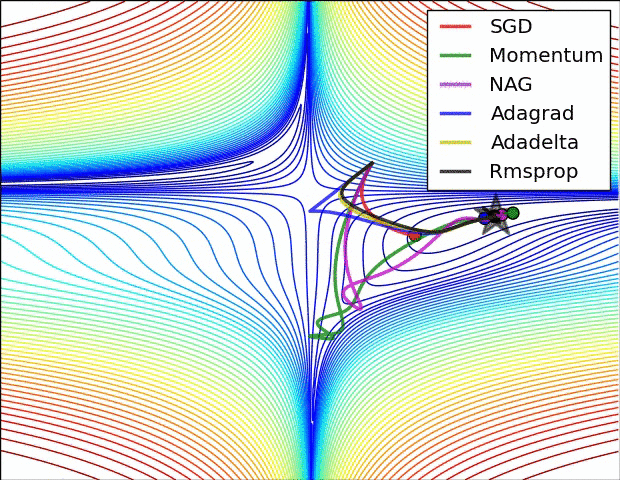
\includegraphics[width=0.8\linewidth]{images/contours_evaluation_optimizers_final_frame.png}
        \caption{SGD optimization on loss surface contours}
        \label{fig:contours_evaluation_optimizers}
    \end{subfigure}%
    \begin{subfigure}{0.5\textwidth}
        \centering
        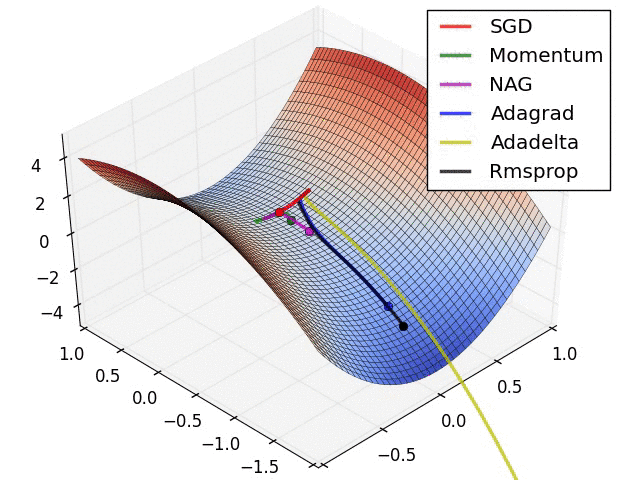
\includegraphics[width=0.8\linewidth]{images/saddle_point_evaluation_optimizers_frame.png}
        \caption{SGD optimization on saddle point}
        \label{fig:saddle_point_evaluation_optimizers}
    \end{subfigure}
    \caption{Source and full animations: \href{http://imgur.com/a/Hqolp}{Alec Radford}}
\end{figure}

As we can see, the adaptive learning-rate methods, i.e. Adagrad, Adadelta, RMSprop, and Adam are most suitable and provide the best convergence for these scenarios.

从这两张图中我们看到,动态调整学习率的几种方法(Adagrad, Adadelta, RMSprop, 以及 Adam)很适应这几种情况,而且表现良好,收敛迅速。

%\subsection{Which optimizer to use?}
\subsection{到底应该选取那个优化算法呢?}

So, which optimizer should you use? If your input data is sparse, then you likely achieve the best results using one of the adaptive learning-rate methods. An additional benefit is that you will not need to tune the learning rate but will likely achieve the best results with the default value.

所以到底应该选择那个优化算法呢? 如果输入数据有稀疏性,那么可能这些动态调整学习率的算法会比较好。这些方法的另一个优点是,使用者不需要调整学习率,因为它们一般情况下在默认设定下就可以达到最佳效果。

In summary, RMSprop is an extension of Adagrad that deals with its radically diminishing learning rates. It is identical to Adadelta, except that Adadelta uses the RMS of parameter updates in the numinator update rule. Adam, finally, adds bias-correction and momentum to RMSprop. Insofar, RMSprop, Adadelta, and Adam are very similar algorithms that do well in similar circumstances. Kingma et al. \cite{Kingma2015} show that its bias-correction helps Adam slightly outperform RMSprop towards the end of optimization as gradients become sparser. Insofar, Adam might be the best overall choice.

Interestingly, many recent papers use vanilla SGD without momentum and a simple learning rate annealing schedule. As has been shown, SGD usually achieves to find a minimum, but it might take significantly longer than with some of the optimizers, is much more reliant on a robust initialization and annealing schedule, and may get stuck in saddle points rather than local minima. Consequently, if you care about fast convergence and train a deep or complex neural network, you should choose one of the adaptive learning rate methods.

\section{Parallelizing and distributing SGD} \label{sec:parallelizing}

Given the ubiquity of large-scale data solutions and the availability of low-commodity clusters, distributing SGD to speed it up further is an obvious choice.
SGD by itself is inherently sequential: Step-by-step, we progress further towards the minimum. Running it provides good convergence but can be slow particularly on large datasets. In contrast, running SGD asynchronously is faster, but suboptimal communication between workers can lead to poor convergence. Additionally, we can also parallelize SGD on one machine without the need for a large computing cluster. The following are algorithms and architectures that have been proposed to optimize parallelized and distributed SGD.

\subsection{Hogwild!}

Niu et al. \cite{Niu2011} introduce an update scheme called Hogwild! that allows performing SGD updates in parallel on CPUs. Processors are allowed to access shared memory without locking the parameters. This only works if the input data is sparse, as each update will only modify a fraction of all parameters. They show that in this case, the update scheme achieves almost an optimal rate of convergence, as it is unlikely that processors will overwrite useful information.

\subsection{Downpour SGD}

Downpour SGD is an asynchronous variant of SGD that was used by Dean et al. \cite{Dean2012} in their DistBelief framework (the predecessor to TensorFlow) at Google. It runs multiple replicas of a model in parallel on subsets of the training data. These models send their updates to a parameter server, which is split across many machines. Each machine is responsible for storing and updating a fraction of the model's parameters. However, as replicas don't communicate with each other e.g. by sharing weights or updates, their parameters are continuously at risk of diverging, hindering convergence.

\subsection{Delay-tolerant Algorithms for SGD}

McMahan and Streeter \cite{Mcmahan2014} extend AdaGrad to the parallel setting by developing delay-tolerant algorithms that not only adapt to past gradients, but also to the update delays. This has been shown to work well in practice.

\subsection{TensorFlow}

TensorFlow\footnote{\url{https://www.tensorflow.org/}} \cite{Abadi2015a} is Google's recently open-sourced framework for the implementation and deployment of large-scale machine learning models. It is based on their experience with DistBelief and is already used internally to perform computations on a large range of mobile devices as well as on large-scale distributed systems. The distributed version, which was released in April 2016 recently in April 2016\footnote{\url{http://googleresearch.blogspot.ie/2016/04/announcing-tensorflow-08-now-with.html}} relies on a computation graph that is split into a subgraph for every device, while communication takes place using Send/Receive node pairs.

\subsection{Elastic Averaging SGD}

Zhang et al. \cite{Zhang2014} propose Elastic Averaging SGD (EASGD), which links the parameters of the workers of asynchronous SGD with an elastic force, i.e. a center variable stored by the parameter server. This allows the local variables to fluctuate further from the center variable, which in theory allows for more exploration of the parameter space. They show empirically that this increased capacity for exploration leads to improved performance by finding new local optima.

\section{Additional strategies for optimizing SGD} \label{sec:strategies}

Finally, we introduce additional strategies that can be used alongside any of the previously mentioned algorithms to further improve the performance of SGD. For a great overview of some other common tricks, refer to \cite{LeCun1998}.

\subsection{Shuffling and Curriculum Learning} \label{sec:shuffling}

Generally, we want to avoid providing the training examples in a meaningful order to our model as this may bias the optimization algorithm. Consequently, it is often a good idea to shuffle the training data after every epoch. 

On the other hand, for some cases where we aim to solve progressively harder problems, supplying the training examples in a meaningful order may actually lead to improved performance and better convergence. The method for establishing this meaningful order is called Curriculum Learning \cite{Bengio2009a}. 

Zaremba and Sutskever \cite{Zaremba2014a} were only able to train LSTMs to evaluate simple programs using Curriculum Learning and show that a combined or mixed strategy is better than the naive one, which sorts examples by increasing difficulty.

\subsection{Batch normalization}

To facilitate learning, we typically normalize the initial values of our parameters by initializing them with zero mean and unit variance. As training progresses and we update parameters to different extents, we lose this normalization, which slows down training and amplifies changes as the network becomes deeper.

Batch normalization \cite{Ioffe2015a} reestablishes these normalizations for every mini-batch and changes are back-propagated through the operation as well. By making normalization part of the model architecture, we are able to use higher learning rates and pay less attention to the initialization parameters. Batch normalization additionally acts as a regularizer, reducing (and sometimes even eliminating) the need for Dropout.

\subsection{Early stopping}

According to Geoff Hinton: ``Early stopping (is) beautiful free lunch''\footnote{NIPS 2015 Tutorial slides, slide 63,  \url{http://www.iro.umontreal.ca/~bengioy/talks/DL-Tutorial-NIPS2015.pdf}}. You should thus always monitor error on a validation set during training and stop (with some patience) if your validation error does not improve enough.

\subsection{Gradient noise}

Neelakantan et al. \cite{Neelakantan2015} add noise that follows a Gaussian distribution $N(0, \sigma^2_t)$ to each gradient update:

\begin{equation}
g_{t, i} = g_{t, i} + N(0, \sigma^2_t)
\end{equation}

They anneal the variance according to the following schedule:
\begin{equation}
\sigma^2_t = \frac{\eta}{(1 + t)^\gamma}
\end{equation}

They show that adding this noise makes networks more robust to poor initialization and helps training particularly deep and complex networks. They suspect that the added noise gives the model more chances to escape and find new local minima, which are more frequent for deeper models.

\section{Conclusion}

In this blog post, we have initially looked at the three variants of gradient descent, among which mini-batch gradient descent is the most popular. We have then investigated algorithms that are most commonly used for optimizing SGD: Momentum, Nesterov accelerated gradient, Adagrad, Adadelta, RMSprop, Adam, as well as different algorithms to optimize asynchronous SGD. Finally, we've considered other strategies to improve SGD such as shuffling and curriculum learning, batch normalization, and early stopping.

\bibliography{overview_sgd}
\bibliographystyle{plain}

\end{document}
